\section{Design}

Review and evaluation of Ohmage reference application and open mHealth schema.
Review case studies. 
Design and prototype alternative trust / security approach to current OAuth2-based mechanism. 
Design new repository. 
Provide NDN-CCL and NFD support for Android. 
Trying replacing REST backend in Ohmage with NDN.

\paragraph{Challenges}

For this application in particular, NDN provides much more relevant functionality at the network layer than IP.  
So solutions in NDN have much more direct impact on the scalability, security, and ease of development; we need not build up additional layers on IP to get near the app challenges.

Cite hourglass figure 

\begin{itemize}
\item Namespace / schema design
\item Repository / storage design
\item Service composability
\item Authentication / identity assurance
\item Data provenance
\item Access auditing
\item Mobile publishing
\item Legal requirements for success
\end{itemize}


\paragraph{Approach}
Follow up on mHealth design approach from Estrin \& Sim, 2010.

\begin{itemize}
\item \textbf{Interoperable, Internet-inspired data exchange} as the backbone of the application ecosystem
\item \textbf{Thin waist of open data interchange standards} that will enable an ecosystem of sensing, storage, analysis, and user interface components to support medical discovery and evidence-based care 
\item Market-supported, patient-centered landscape of innovative health applications
\item \textbf{Patient-controlled, privacy-aware data exchange} across device, component, and application boundaries
\end{itemize}

\paragraph{mHealth Reality Check}

%% From 
%% PLOS Medicine Editors. "A reality checkpoint for mobile health: three challenges to overcome." PLoS Medicine 10.2 (2013).
%% TODO: Add to cites

\begin{itemize}
\item \textbf{Are your systems interoperable?}
Estrin \& Sim in Science, 2010.  Open mHealth. 
\item \textbf{Are you using open standards?}
WHO, 2013.  eHealth unit. 
\item \textbf{How will you evaluate?}
Greenhalgh et al. in BMC Med Res. Methodology, 2011.
Realist and meta-narrative evidence synthesis.
\end{itemize}

\subsection{Reference Application: Ohmage} 

Plan to create/port a mobile client for the Ohmage reference platform, which currently incorporates:
Mobile application, LAMP stack back-end, REST communication

Key pain point is OAuth 2.0:  Implementation relies on this � doesn�t scale to the DPU model and has numerous problems.  Quickly identified by 

Open mHealth lead architect as a primary challenge.   

Same approach (apparently) used in Human API mentioned earlier. 


\subsection{User Interface}
Begin with this, because consumer-facing. 

\subsubsection{Mobile}
\subsubsection{Website}
Start with Ohmage front end (see previous slides).
Web-based front end using NDN-JS to access derived data without location information.
Examples: http://quantifiedself.com/fitbit/ 



\subsection{NDNEx Application architecture}

Translate existing REST-based approach?  How quickly to move to a new model of data exchange where transactions are mostly about (for example) keys. 

Based on 
PEIR, the personal environmental impact report, as a platform for participatory sensing systems research. Mun, M., Reddy, S., Shilton, K., Yau, N., Burke, J., Estrin, D., ... \& Boda, P. (2009, June). Proc. ACM Mobisys 2009. 

  
Capture (Anyang / Tsinghua / UCLA) 
Storage (Tsinghua / UCLA)
Processing (Basel)
Presentation (REMAP)
Security (Michigan)


\subsection{Trust and security}

Replacing Oauth2 for distributed processing is critical

\subsubsection{Trust model} 
Leverage PKI as deployed

\subsubsection{Identity}
Each processing block in this diagram may come from a different service provider. 
User may have different identity per service (or at least per flow). 
Each step tends to generate derived data that must also be stored and may not be associated with the original identity.  

\subsubsection{Integrity} 

\subsubsection{Confidentiality}
Access control in "data flow" model for communication between processing components, replacing Oauth (with Tsinghua and UCLA).  Extensions to support epidemiological studies incorporating semi-anonymized opt-in data across large populations. 

Name privacy considerations.


\subsection{Naming}

\subsubsection{Data}
Personal health data (and metadata) namespace and repository design � focusing on support for physical activity data in the first round.  
What schema? Initially, try direct mapping of Open mHealth schema to names

\subsubsection{Certificates}

\subsubsection{Processing}
Borrow ideas from Named Function Networking concept for distributed processing


\subsection{Storage}

(Hierarchical network of repositories, similar to BAS/BMS, including both personal repositories, service provider backups for personal data, and aggregated "anonymized" stores). 



\subsection{Routing \& Forwarding}
Mobile publishing support



\begin{figure}
\centering
\subfigure[Mobile publisher connected to ``home'' hub, which directly routes its publishing prefix.]{
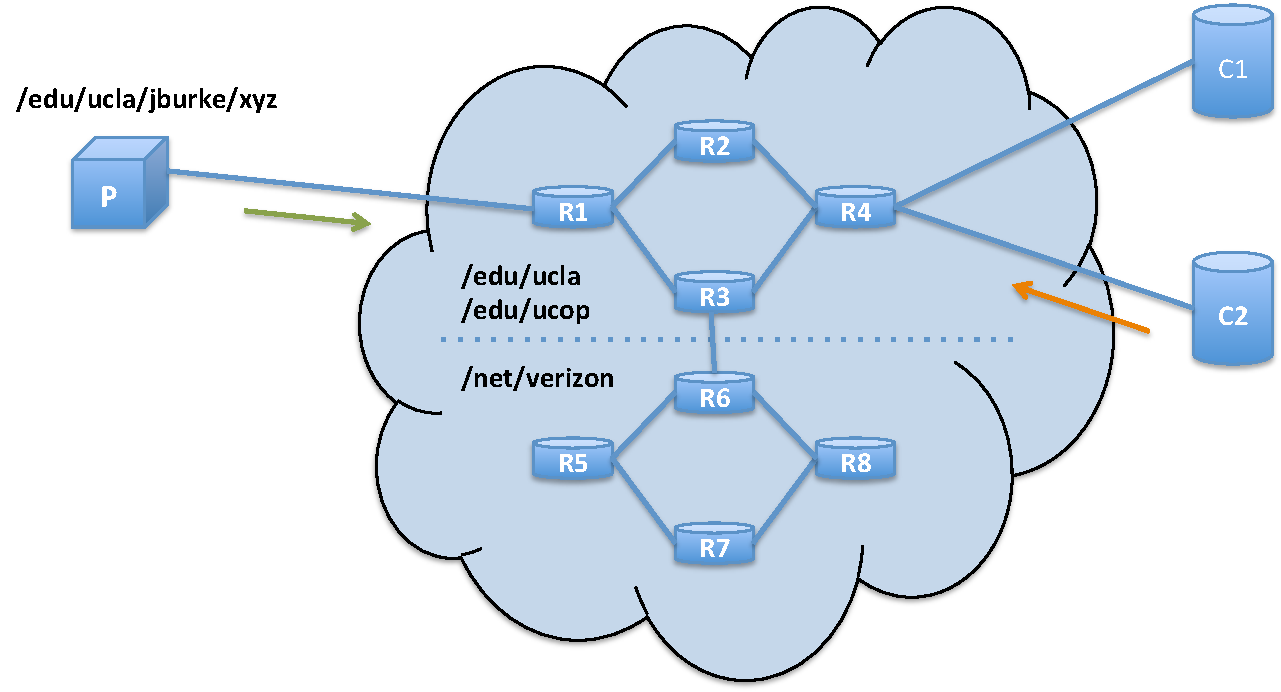
\includegraphics[width=0.45\columnwidth, keepaspectratio=true]{figures/publisher-mobility-a}
}
\subfigure[Mobile publisher connected to another hub, which does not directly route its prefix.]{
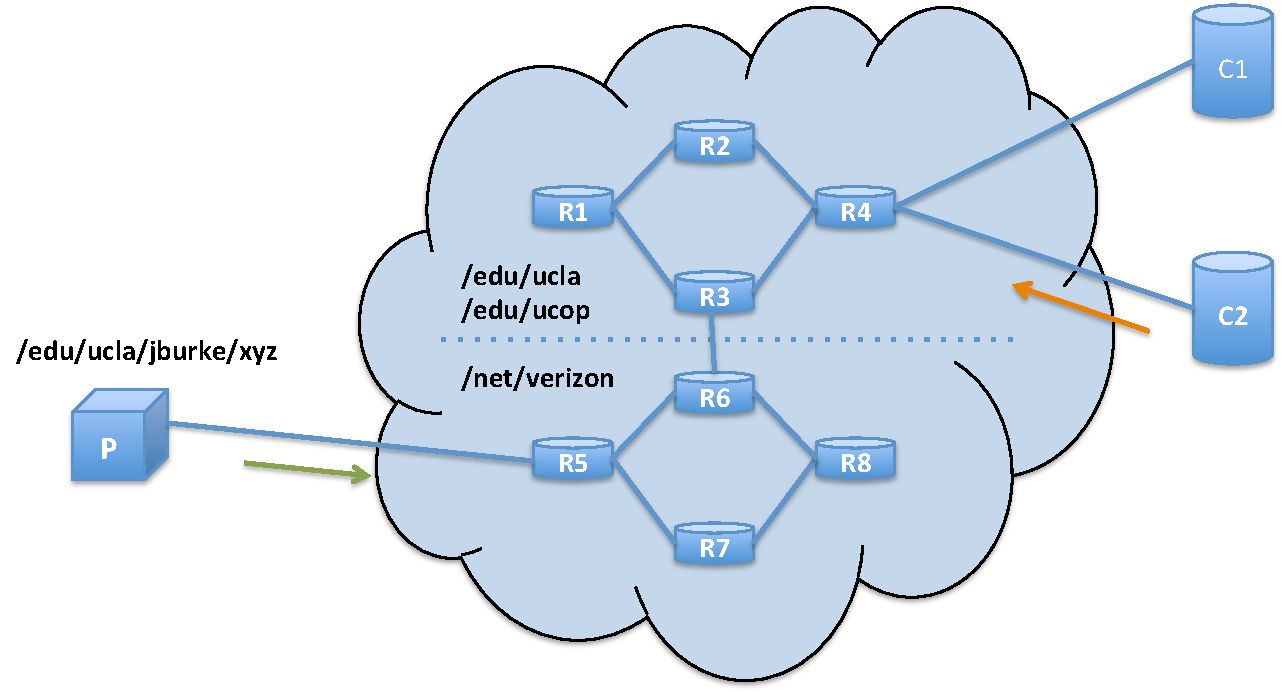
\includegraphics[width=0.45\columnwidth, keepaspectratio=true]{figures/publisher-mobility-b}
}
\caption{Mobile publisher scenario.}
\label{fig:mobilepublisher}
\end{figure}

\subsection{Distributed Processing}
Incorporate Haitao's design?
Named Function Networking style support for distributed processing with University of Basel. 

